\section{Module d'IA générative hybride (RAG local et agent cloud)}
\label{chap:ia_rag}

Cette section décrit le module qui porte la contribution la plus distinctive de la plateforme : un agent conversationnel hybride, au sens défini en introduction. Un service local auto-hébergé (Mistral~7B via Ollama) traite les requêtes sensibles, qui doivent rester sous le contrôle de l'entreprise. Un service cloud (\texttt{claude-sonnet-4-5}, API Anthropic) traite les requêtes analytiques non sensibles, qui demandent une plus grande capacité de raisonnement. Nous décrivons ici la construction des deux chemins et du mécanisme qui les arbitre ; leur évaluation comparative, qui porte l'hypothèse H2, fait l'objet de la section~\ref{chap:benchmark_rag}.

\subsection{Architecture d'ensemble du module conversationnel hybride}
\label{sec:ia_archi}

Une requête suit toujours le même trajet. L'utilisateur la saisit dans le panneau conversationnel, ouvert par le bouton \textit{Assistant IA} de l'application (Figure~\ref{fig:ui_dashboard}). Un proxy de l'API Express la relaie à l'orchestrateur n8n, qui en évalue la sensibilité et la route vers l'un des deux chemins. L'échange est ensuite journalisé, quel que soit le chemin emprunté. Ce trajet est celui de la Figure~\ref{fig:seq_rag} (séquence) et de la Figure~\ref{fig:c4_conteneurs} (conteneurs) ; cette section en détaille l'implémentation.

\textbf{n8n comme point d'orchestration unique.} C'est le workflow n8n, et non l'application Express ou le service FastAPI, qui porte la logique hybride : il reçoit chaque requête, en évalue la sensibilité et décide du chemin (\texttt{EF-RAG-03}, ADR-02, \S\ref{sec:adr}). Les deux chemins augmentent la génération par des données métier réelles, mais par des mécanismes de récupération différents. Côté cloud (\S\ref{sec:ia_cloud}), un agent génère lui-même une requête SQL sur les vues relationnelles de la base. Côté local (\S\ref{sec:ia_local}), c'est le code du service qui récupère les données : par des filtres SQL déterministes (plaque, période, mots-clés) d'abord, par similarité vectorielle sur le corpus produit par l'ETL (\S\ref{sec:  vectorisation}) en dernier recours. Les deux relèvent du paradigme RAG au sens large : récupérer un contexte pertinent avant de générer.

\textbf{Le proxy Express.} Les routes qui relaient la requête vers n8n vivent dans le dépôt applicatif (section~\ref{chap:webapp}), mais relèvent de ce module. \texttt{POST~/api/chat} (\texttt{routes/chat.js}) est la route utilisée par le panneau conversationnel. Elle valide le message, le relaie au \textit{webhook} n8n avec un délai d'attente dimensionné pour les itérations d'un agent outillé, normalise la réponse et journalise l'échange dans \texttt{chat\_messages} (\S\ref{sec:ia_tracabilite}). Elle transmet aussi au client le chemin emprunté (\texttt{local} ou \texttt{cloud}), que l'interface affiche sous chaque réponse. \texttt{GET~/api/chat/history} expose l'historique d'un utilisateur. La route \texttt{POST~/api/analyze} (\texttt{index.js}) relaie elle aussi vers n8n, mais aucun composant du frontend ne l'appelle : c'est du code mort, que nous signalons comme tel.

\subsection{Le service RAG local souverain}
\label{sec:ia_local}

Le service FastAPI du chemin local est celui qui incarne le plus directement la souveraineté visée par H2 : un RAG conversationnel sur un corpus métier français, sans dépendance à un service tiers. Nous l'avons construit selon le schéma \textit{retriever--augmentation--generator} de Lewis et al. \cite{lewisRetrievalaugmentedGenerationKnowledgeintensive2020} (\S\ref{sec:Systemes_RAG_IA_Generative}), adapté à un corpus structuré et très redondant.

\subsubsection{Le retrieval : SQL exact d'abord, vectoriel en dernier recours}

\texttt{fetch\_rows()} applique une stratégie par passes successives. Elle repose sur une hypothèse simple : une correspondance exacte sur un identifiant métier (une plaque, une période, un mot du domaine) est un signal plus fiable qu'une similarité sémantique.

\begin{itemize}
    \item \textbf{Passe~0, la plaque.} Une immatriculation détectée dans la question filtre la vue \texttt{v\_transactions\_completes} sur la colonne \texttt{camion}, éventuellement croisée avec la période. Elle est prioritaire et isolée des autres mots-clés, pour ne pas diluer ce signal fort (« CAMION » figure dans des centaines de libellés sans rapport avec le véhicule visé).
    \item \textbf{Passes~1 et~2, les mots-clés.} Vingt et un mots déclencheurs du domaine (\textit{ex.} \texttt{CARBURANT}, \texttt{VIDANGE}, \texttt{RATION}) sont cherchés dans les libellés, d'abord en conjonction stricte, puis en disjonction. Certains sont traduits vers le vocabulaire réel de la base : « amende » ne figure dans aucun libellé, ce sont « contravention », « pesage » ou « défaut de papier » qui y figurent.
    \item \textbf{Filtres transverses.} Une période exprimée en toutes lettres (« mars 2026 », « T1 2026 ») ou au format ISO, et des critères de flotte (pays, type de propriété, statut) s'ajoutent en conjonction à toutes les passes. Si une question filtrée ne trouve rien, le service répond « aucune donnée » plutôt que de se replier sur une recherche vectorielle qui ignorerait le filtre.
    \item \textbf{Passe~3, le repli vectoriel.} Seulement si tout le reste échoue : la question est encodée par le même modèle qu'à l'ingestion (\texttt{all-MiniLM-L6-v2} \cite{reimersSentencebertSentenceEmbeddings2019}), puis comparée à \texttt{transport\_embeddings} par similarité cosinus (opérateur \texttt{<=>} de \texttt{pgvector}), qui renvoie les $k=10$ passages les plus proches \cite{karpukhinDensePassageRetrieval2020}.
\end{itemize}

\begin{lstlisting}[language=SQL, basicstyle=\ttfamily\footnotesize, breaklines=true, showstringspaces=false]
SELECT date, libelle, sortie FROM transport_embeddings
ORDER BY embedding <=> %s::vector ASC LIMIT 10
\end{lstlisting}

\textbf{Des réponses exactes sans modèle de langage.} Les LLM sont peu fiables en arithmétique. Nous avons donc retiré au modèle tout calcul qu'une requête SQL peut faire. Pour les passes~0 à~2, le total et le nombre d'opérations sont calculés par \texttt{SUM} et \texttt{COUNT} sur \emph{toutes} les lignes qui correspondent au filtre, pas seulement sur les dix transmises au modèle. Trois familles de questions sont ensuite servies directement, sans appel au LLM :
\begin{itemize}
    \item les comptages de camions (« combien de camions maliens actifs ? »), par un \texttt{COUNT} SQL ;
    \item le solde de caisse, calculé selon la même définition que la carte « Solde actuel » du tableau de bord ;
    \item les demandes d'agrégat (« total », « somme », « combien »), qui reçoivent le total SQL déjà calculé.
\end{itemize}
Pour les autres questions, le total est placé en tête du contexte, avec la mention « TOTAL EXACT (déjà calculé, à recopier tel quel) ». Pour le repli vectoriel, qui n'a pas de filtre exploitable, la mention devient « TOTAL APPROXIMATIF ». La part des questions du benchmark servies sans LLM est mesurée à la section~\ref{chap:benchmark_rag}.

\subsubsection{La génération}

Les questions ouvertes sont transmises à Mistral~7B par l'API de conversation d'Ollama (\texttt{http://ollama:11434/api/chat}), sous forme d'un message système et d'un message utilisateur contenant le contexte. Le message système impose une réponse en français de trois ou quatre phrases, la recopie mot pour mot du total fourni, la citation de deux ou trois postes de dépense représentatifs et l'aveu explicite d'une information absente. Nous avons fixé la température à~0,1, pour des réponses stables d'un appel à l'autre, et limité la sortie à 300~jetons. Le nom du modèle (\texttt{mistral:latest}) est écrit en dur dans la requête, et le message système est dupliqué entre les deux fonctions de génération : deux dettes de maintenabilité (\texttt{ENF-MAINT-01}, \texttt{ENF-MAINT-02}) reprises au §\ref{sec:ia_dettes}.

\subsubsection{Les points d'entrée}

Le service expose deux \textit{endpoints}, authentifiés par l'en-tête \texttt{X-API-Key} : \texttt{POST~/ask} renvoie la réponse complète en un bloc JSON ; \texttt{POST~/ask/stream} la restitue jeton par jeton. Le streaming répond à une contrainte d'usage : sans accélération matérielle (ADR-03, \S\ref{sec:adr}), l'inférence est lente, et une réponse qui se construit progressivement vaut mieux qu'un long silence. Un \textit{endpoint} \texttt{/health}, public et sans donnée, sert au contrôle de santé du conteneur (Figure~\ref{fig:ia_rag_api_logs}).

\begin{figure}[H]
    \centering
    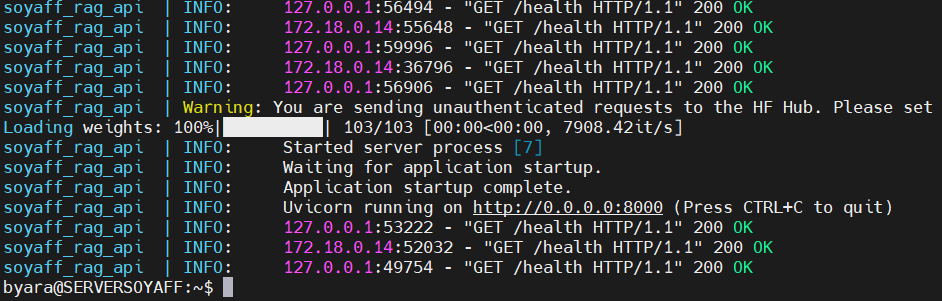
\includegraphics[width=0.65\textwidth]{figures/captures/ia_rag_api_logs.png}
    \caption{Démarrage du service RAG local en production et sondes de santé périodiques}
    \label{fig:ia_rag_api_logs}
\end{figure}

\textbf{Souveraineté par construction.} Sur ce chemin, aucune donnée de la base ne sort du serveur : le \textit{retrieval} interroge PostgreSQL en local, l'inférence s'exécute dans le conteneur Ollama du même réseau Docker, et seule la réponse finale est renvoyée à n8n. Cette étanchéité réalise \texttt{ENF-SOUV-01} pour ce chemin ; c'est un fait de construction, pas encore une mesure.

\subsection{Le chemin cloud}
\label{sec:ia_cloud}

Le second chemin traite les requêtes analytiques non sensibles (\texttt{EF-RAG-01}, \texttt{EF-RAG-02}) : agrégations, comparaisons temporelles, classements sur l'ensemble du référentiel. Pour ces requêtes, la capacité de raisonnement d'un grand modèle l'emporte sur la contrainte de souveraineté (\S\ref{sec:Systemes_RAG_IA_Generative}).

\textbf{Le modèle et son emplacement.} Le modèle est \texttt{claude-sonnet-4-5-}\allowbreak\texttt{20250929} de l'API Anthropic. L'appel n'est fait nulle part dans le code Express : il est porté par un nœud \textit{AI Agent} de n8n (\textit{framework} LangChain), connecté à un nœud de modèle Anthropic. Le proxy applicatif ignore l'existence de ce modèle.

\begin{sloppypar}
\textbf{Un agent outillé.} L'agent dispose d'un outil d'exécution SQL sur PostgreSQL. La requête est générée par le modèle à partir d'un \textit{system prompt} versionné (\texttt{n8n/system\_prompt\_agent.md}), qui documente les vues métier (\texttt{v\_transactions\_completes}, \texttt{v\_stats\_par\_camion}, \texttt{v\_resume\_mensuel}, \texttt{v\_stats\_par\_produit}), les conventions du domaine et des exemples de correspondance question--requête. Une mémoire conversationnelle, également dans PostgreSQL, conserve les dix derniers échanges d'une session : l'agent peut ainsi résoudre « ce camion » dans une question de relance. La réponse suit un gabarit imposé : tableau, analyse, recommandation le cas échéant.
\end{sloppypar}

\textbf{Un accès en lecture seule.} Le SQL généré par un modèle ne doit pas pouvoir modifier la base. Nous avons donc connecté l'outil SQL à un rôle PostgreSQL dédié, \texttt{soyaff\_agent\_ro} (migration Alembic~004). Ses sessions sont en lecture seule par défaut, ses requêtes sont interrompues au-delà de 15~secondes et il ne peut ouvrir que cinq connexions. Il ne lit que les tables et vues métier ; la table \texttt{chauffeurs} (noms, téléphones), les embeddings et l'historique des conversations lui sont inaccessibles. La mémoire de conversation utilise un autre compte. La garantie ne repose donc plus sur l'obéissance du modèle aux consignes, mais sur les droits de la base (voir le test du §\ref{sec:test_bout_en_bout}).

\textbf{Une frontière franchie.} Ce chemin traverse le périmètre souverain de la Figure~\ref{fig:c4_conteneurs} : la question de l'utilisateur et les résultats des requêtes SQL de l'agent sont traités par un service tiers. Le routage décrit ci-dessous existe pour limiter ce franchissement aux requêtes non sensibles.

\subsection{Le routage par sensibilité}
\label{sec:ia_routage}

Le routage est le mécanisme qui fait exister l'hybride au sens de l'introduction ; il réalise \texttt{EF-RAG-03}. Chaque requête entre dans le workflow n8n de la Figure~\ref{fig:ia_workflow}, dont le premier nœud de code en évalue la sensibilité. Une requête sensible part vers le service local par une requête HTTP authentifiée (\texttt{POST~http://api:8000/ask}) ; une requête non sensible est confiée à l'agent cloud. Nous avons formalisé cette décision dans l'\texttt{ADR-02} (\S\ref{sec:adr}) : un point de décision unique plutôt qu'une logique dispersée dans chaque service.

\begin{figure}[H]
    \centering
    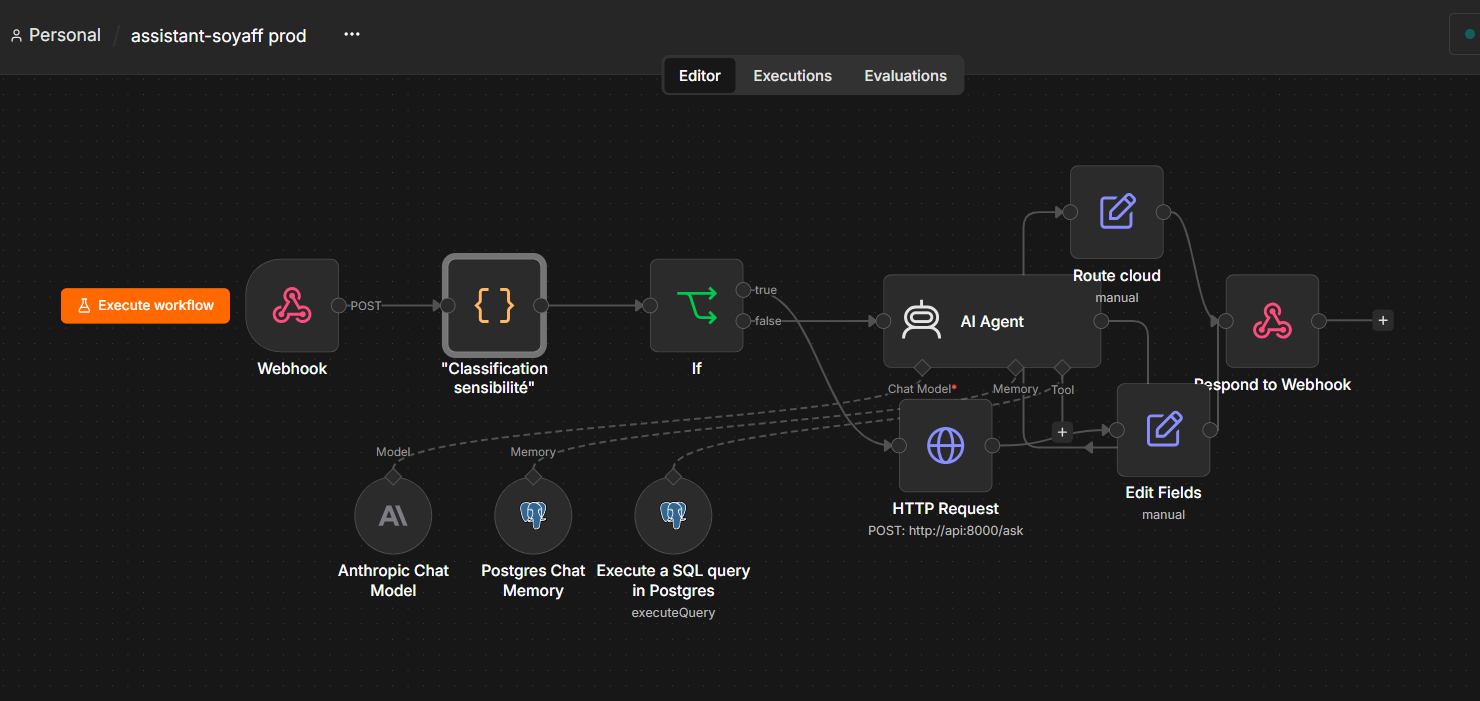
\includegraphics[width=0.85\textwidth]{figures/captures/ia_workflow_n8n.png}
    \caption{Workflow n8n de routage hybride en production}
    \label{fig:ia_workflow}
\end{figure}

\textbf{Le mécanisme.} La classification est une heuristique par mots entiers et expressions régulières, appliquée à la question débarrassée de ses accents et mise en majuscules (Figure~\ref{fig:ia_classifieur}). Ce n'est pas un classifieur d'apprentissage automatique, ainsi que l'assume l'\texttt{ADR-02}. Deux règles décident :
\begin{itemize}
    \item toute mention d'\textbf{identité} reste locale, même dans une question d'agrégat : un terme comme \textit{chauffeur}, \textit{salaire}, \textit{paie}, \textit{téléphone}, \textit{CNI} ou \textit{adresse}, ou une plaque d'immatriculation (« total du camion AA~076~AH », « top des chauffeurs ») ;
    \item un \textbf{montant financier précis} (\textit{solde}, \textit{reliquat}, \textit{avance}, « combien doit ») reste local, \emph{sauf} si la question est explicitement agrégée (\textit{total}, \textit{moyenne}, \textit{comparaison}, \textit{tendance}, \textit{top}, \textit{classement}, \textit{évolution}, pourcentage).
\end{itemize}
La seconde règle traduit un choix assumé : tout le métier de SOYAFF est financier, et classer sensible toute mention de montant viderait le chemin cloud de son utilité. La recherche par mot entier évite les faux déclencheurs (« TOP » dans « STOP », « PAIE » dans « PAIEMENT »), et le motif de plaque écarte les faux positifs du français courant (« EN 2025 », « DE 1500 »).

\begin{figure}[H]
    \centering
    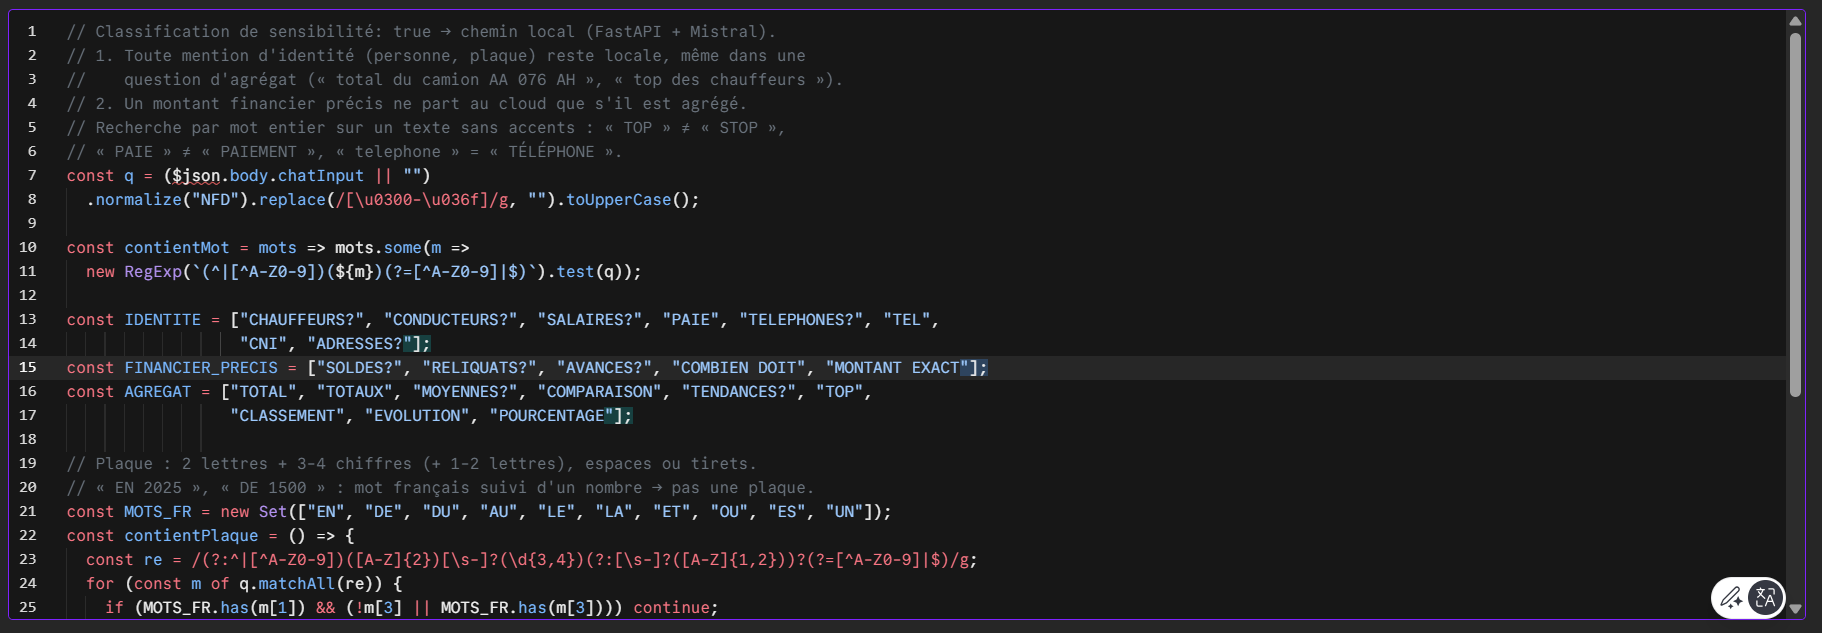
\includegraphics[width=0.9\textwidth]{figures/captures/ia_classifieur.png}
    \caption{Règles du classifieur de sensibilité (nœud de code n8n, extrait)}
    \label{fig:ia_classifieur}
\end{figure}

\textbf{Le routage vérifié.} Les Figures~\ref{fig:ia_route_locale} et~\ref{fig:ia_route_cloud} montrent les deux chemins en production. Une question sur les dépenses d'un camion identifié est traitée en local : la réponse est un total SQL exact, sans appel au LLM. Une question agrégée sur la flotte est traitée par l'agent cloud, qui répond par un tableau, une analyse et des recommandations. L'étiquette affichée sous chaque réponse indique le chemin emprunté, jamais le modèle utilisé.

\begin{figure}[H]
    \centering
    \begin{minipage}[t]{0.48\textwidth}
        \centering
        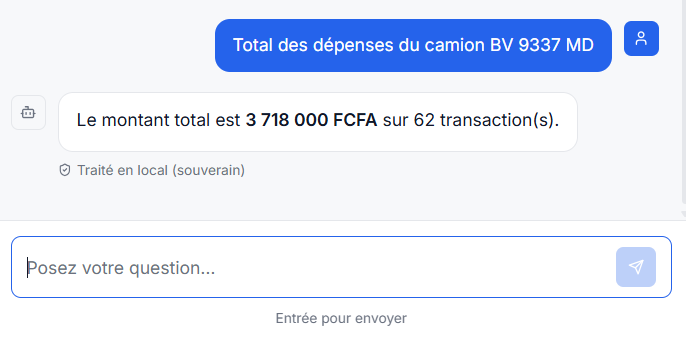
\includegraphics[width=\textwidth]{figures/captures/ia_route_locale.png}
        \caption{Question portant sur un camion identifié : traitée en local (souverain)}
        \label{fig:ia_route_locale}
    \end{minipage}\hfill
    \begin{minipage}[t]{0.48\textwidth}
        \centering
        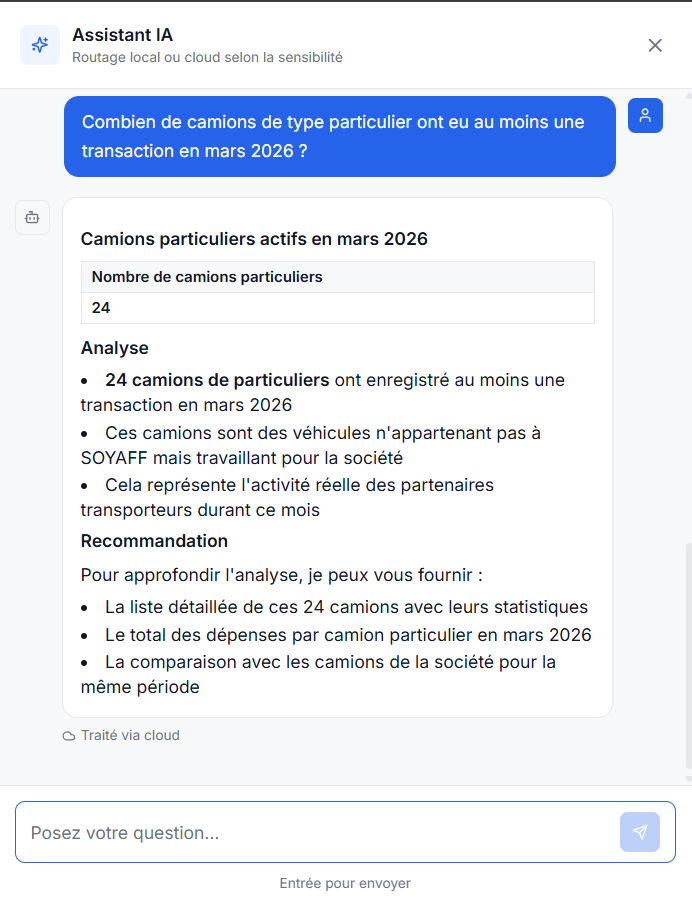
\includegraphics[width=\textwidth]{figures/captures/ia_route_cloud.png}
        \caption{Question agrégée sur la flotte : traitée via le cloud}
        \label{fig:ia_route_cloud}
    \end{minipage}
\end{figure}

\textbf{Une limite résiduelle.} L'heuristique reste lexicale. Un nom de chauffeur cité seul, sans le mot « chauffeur » ni plaque, n'est pas détecté : la requête part vers le cloud. Le risque est borné par le rôle en lecture seule (\S\ref{sec:ia_cloud}) : l'agent n'a pas accès à la table \texttt{chauffeurs} et ne peut donc pas associer ce nom à des données personnelles. Le workflow est versionné dans le dépôt \texttt{assistant-soyaff-1} (\texttt{n8n/assistant-soyaff-hybrid-routing.json}) : la classification, les deux branches et leur authentification sont reproductibles indépendamment de l'instance n8n en production.

\textbf{La conséquence méthodologique.} L'hypothèse H2 porte sur la parité d'exactitude entre les deux \emph{services d'inférence}, pas sur la justesse du classifieur qui choisit entre eux. Mesurer H2 à travers le chemin réellement emprunté par n8n ferait dépendre le résultat de la précision du classifieur, une autre question. Le benchmark de la section~\ref{chap:benchmark_rag} interroge donc chaque service directement, sur le même jeu de questions. La validité du classifieur est un chantier d'évaluation distinct, non couvert par H2.

\subsection{Citation des sources et journalisation}
\label{sec:ia_tracabilite}

\textbf{Citation des sources (EF-RAG-04) : une transparence sur le contexte.} Le service local renvoie, à côté de la réponse, les lignes qui ont servi à la construire (date, libellé, montant) et le total exact : dans le champ \texttt{context} de \texttt{/ask}, et dans l'en-tête \texttt{X-RAG-Context} de \texttt{/ask/stream}. C'est une transparence sur le contexte, pas une citation au sens strict : aucune affirmation du texte généré n'est reliée à un enregistrement précis. Côté cloud, le \textit{system prompt} ne demande pas de citation ; le tableau que l'agent inclut dans sa réponse montre les lignes renvoyées par sa requête SQL, sans mécanisme de citation formalisé. \texttt{EF-RAG-04} est donc partiellement réalisée.

\textbf{Journalisation (EF-RAG-05) : uniforme, en aval du routage.} Chaque échange est consigné dans \texttt{chat\_messages} (\texttt{user\_id}, \texttt{role}, \texttt{content}, \texttt{created\_at}) par le proxy Express : le message de l'utilisateur, puis la réponse, quel que soit le chemin qui l'a produite. Cette journalisation sert la piste d'audit exigée par \texttt{ENF-SEC-04} et constitue un corpus de questions réelles utile à l'évaluation. La mémoire conversationnelle de l'agent cloud (\S\ref{sec:ia_cloud}) est un mécanisme distinct : elle sert la continuité d'une session, sans les métadonnées d'audit ni l'exhaustivité exigées par \texttt{EF-RAG-05}.

\subsection{Écarts, dettes et cohérence}
\label{sec:ia_dettes}

Nous rassemblons ici les écarts du volet IA ; leur priorisation est discutée à la section~\ref{chap:discussion}. Ce sont des dettes de finition et de traçabilité, pas des défauts des moteurs d'inférence : les deux chemins existent, répondent et sont arbitrés par le routage.

\begin{itemize}
    \item \textbf{\texttt{ENF-MAINT-01} : pas d'interface d'inférence abstraite.} Le nom du modèle local est écrit en dur dans l'appel à Ollama ; changer de modèle impose de modifier le code.
    \item \textbf{\texttt{ENF-MAINT-02} : message système dupliqué} entre les fonctions de génération bloquante et en flux, au lieu d'être factorisé.
    \item \textbf{Citation des sources partielle (\texttt{EF-RAG-04}).} Transparence sur le contexte côté local, aucune citation structurée des enregistrements sur l'un ou l'autre chemin.
    \item \textbf{Classifieur lexical (\texttt{EF-RAG-03}).} Un nom de chauffeur cité seul n'est pas détecté ; le rôle en lecture seule borne le risque sans le supprimer.
\end{itemize}

Plusieurs dettes relevées lors de la première rédaction ont été refermées depuis. L'outil SQL de l'agent cloud n'avait aucun garde-fou technique : il utilise désormais le rôle \texttt{soyaff\_agent\_ro}. Le classifieur envoyait au cloud une question d'agrégat nommant un chauffeur ou un camion : l'identité l'emporte désormais sur l'agrégat. Le total transmis au modèle local ne sommait que les dix lignes affichées : il est calculé en SQL sur toutes les lignes correspondantes. Enfin, le contexte n'était pas exposé en mode streaming : il l'est par l'en-tête \texttt{X-RAG-Context}. L'\texttt{ADR-02} (\S\ref{sec:adr}) signale ces résorptions.

\subsection{Synthèse et transition}

Nous avons construit dans cette section les deux chemins de l'agent conversationnel hybride et le mécanisme qui les arbitre. Le service local (\S\ref{sec:ia_local}) réalise par construction la souveraineté d'\texttt{ENF-SOUV-01} et ne confie au modèle de langage que ce qu'une requête SQL ne sait pas faire. Le chemin cloud (\S\ref{sec:ia_cloud}) s'appuie sur un agent outillé, borné par un rôle en lecture seule. Le routage (\S\ref{sec:ia_routage}) a été vérifié dans les deux sens en production, et le workflow qui le porte est versionné. Nous n'avançons ici aucun chiffre de performance : cette mesure est l'objet de la section~\ref{chap:benchmark_rag}.

Ces modules ne tiennent en production que parce qu'une infrastructure les déploie, les supervise et les maintient disponibles avec des ressources limitées. C'est l'objet de la section suivante.
